\section{Selection Cuts}
\label{sect:cuts}

%{\bf FIXME material for the cut justification/pile up reweithing/BTg SF can appear here.}

In order to select signal events and suppres SM backgrounds, a set of cuts which are listed below, is applied.
\begin{itemize}
\item The preselection cuts which was outlined in Section~\ref{subsect:presel}.
\item Offline trigger cuts mentioned in Section ~\ref{sect:triggerstudy}. They ask for at least 4 jets with $\abs\eta<2.4$
%\item At least 4 jets with $p_T>40$ GeV and $\abs\eta<2.4$ are required which are asked to pass loose pf-jet id cuts.
\item Among these set of jets, first and second leading jets are needed to have a \pT greater than $100$ GeV and $60$ GeV, respectively.
\item It is also required that each jet with \pT $>$ 50 GeV to pass loose pf-jet id cuts.
\item At least one b-quark jet is requested with \pT $>$ 20 GeV within the tracker acceptance, which is tagged by the Combined Secondary Vertex algorithm with a tight working point.
\item The difference between \met and the vectorial \pT sum of the selected jets, electrons and muons should be below $70$ GeV.
\item The \mindphifour of the four leading jets should be greater than 0.3. There is no requirement on the id or \pT of the jets when looking for the minimum azimuthal angle between \met and jets. 
\item \met is required to be greater than $30$ GeV. 
\item Leptons, being either electrons or muons, are vetoed.
\item A cut on \mttwo $>$ 125 GeV is applied.
\end{itemize}

The effect of the selection cuts on different backgrounds is shown is Table \ref{Tab.CutFlow}

\begin{table}[!htb]
\begin{center}
\begin{tabular}{|c|c|c|c|c|c|}
\hline
 Cut                            &      QCD   &$W$+jets & $Z$+jets & Top      & Total \\\hline    %&SUSY &MJ-Data&
 Trigger                        & 5715523.28 & 7307.79 & 2432.95  & 60071.28 &5785335.30$\pm$26646.27\\ %SUSY 718.16   Data  4485758.00
 Jet ID                         & 5713982.08 & 7292.60 & 2432.95  & 60040.64 &5783748.26$\pm$26645.46\\%SUSY  717.67   Data  4484247.00
 Lepton Veto                    & 5709941.35 & 4759.89 & 1855.46  & 51143.85 &5767700.56$\pm$26642.92\\%SUSY  619.95    Data 4469115.00
 BJet                           & 583250.20  & 323.93  &  155.37  & 34252.57 &617982.07$\pm$8690.65\\  %SUSY  447.29   Data 578345.00
 \mindphifour$>$ 0.3            & 310092.56  & 198.38  &  103.58  & 19147.93 &329542.46$\pm$6437.28\\  %SUSY  338.33   Data 318801.00
 $M_{T2} >$ 125                  & 465.73     & 30.99   &   22.92  & 561.55   &1081.19$\pm$121.23\\  %SUSY  150.12  Data  779.00&
 $|\met -MHT| <$ 70             &  72.22     &  27.66  &  20.47   &  470.25  &590.61$\pm$21.63\\  %SUSY  135.45  Data  606.00&
\hline
\end{tabular}
\caption{Event yields after applying different cuts. "Trigger" contains all of the preselections and offline trigger cuts.}
\label{Tab.CutFlow}
\end{center}
\end{table}

\subsection{Cuts Justification}
We performed some checks to justify our analysis cuts. Our cuts were optimised based on maximization of the statistical significance. We studied our main cuts in this analysis.
In Figure \ref{fig:MT2diffVSPT} we show the \mttwo distribution for QCD for different intervals of VSPT. The different distributions 
are normalized to the same area. The variable is plotted for QCD events that
pass the cuts described above. From Figure \ref{fig:MT2diffVSPT}, we see that for
large values of VSPT, the \mttwo distribution is distorted and deviates from the distribution with
$0 <$ VSPT $<20$, i.e. small VSPT. Since the distortion becomes significant for VSPT $> 70$ GeV, we
cut away events above this value. 
\begin{figure}[!Hhtb]
\begin{center}
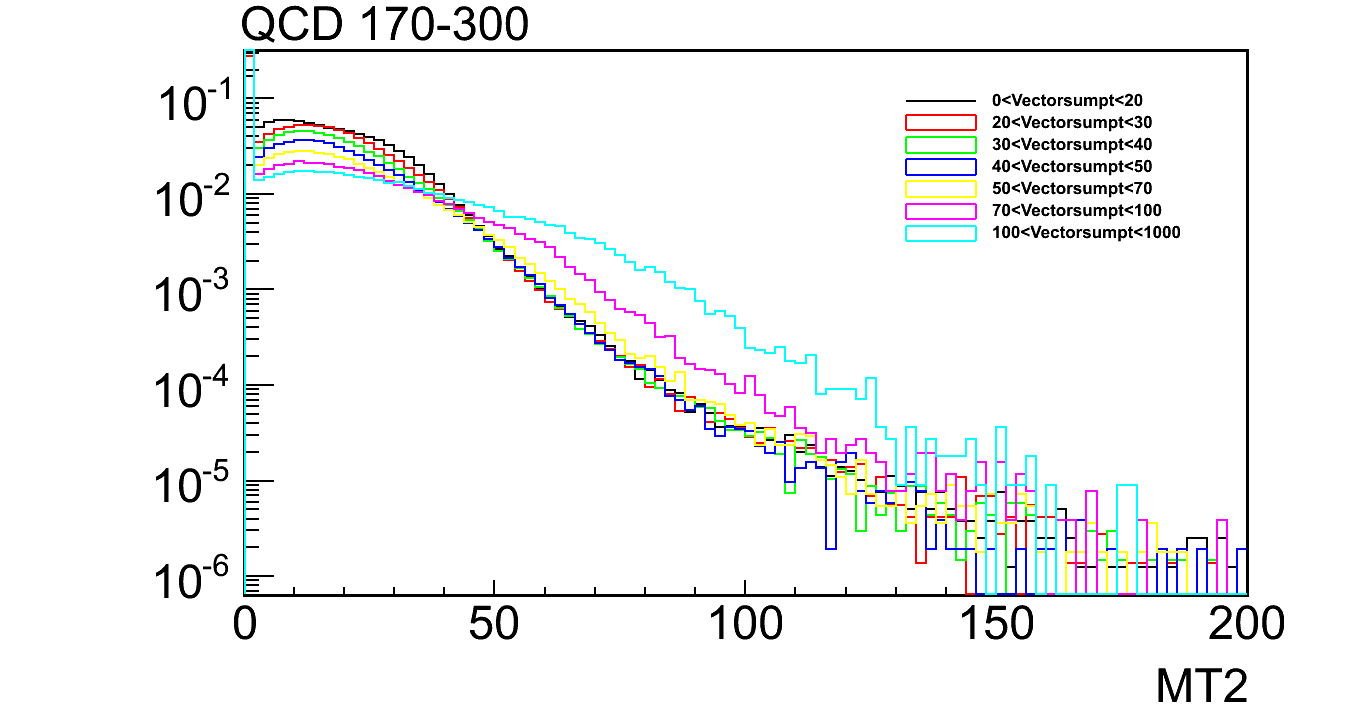
\includegraphics[angle=00,width=0.5\textwidth]{figs/MT2-diffVSPT-QCD170-300.png}\\
%	\mbox{\small{(1)} \\
\end{center}
\caption{Disrtibution of \mttwo in different VSPT ranges for one QCD sample}
\label{fig:MT2diffVSPT}
\end{figure}
  
We looked at the distributions of different variables before and after applying VSPT $<70$ when the other cuts 
except $\mttwo > 125 $ were relaxed. As it is obvious from Figures \ref{fig:MT2VSPT}-\ref{fig:VSPTVSPT}, by applying VSPT $<70$ we have better agreement 
between data and MC,

\begin{figure}[!Hhtb]
\begin{center}$
\begin{array}{cc} 
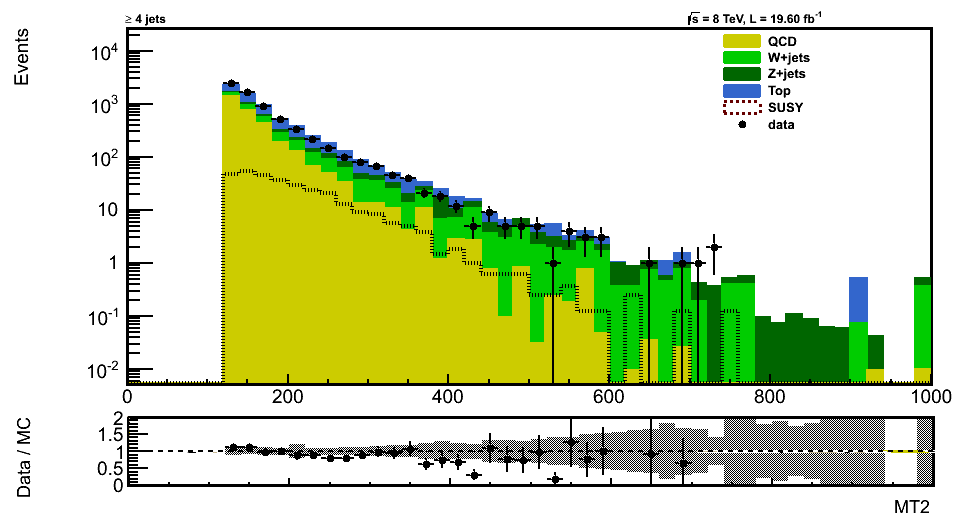
\includegraphics[angle=00,width=0.5\textwidth]{figs/MT2-cut(MT2+trig).png}&
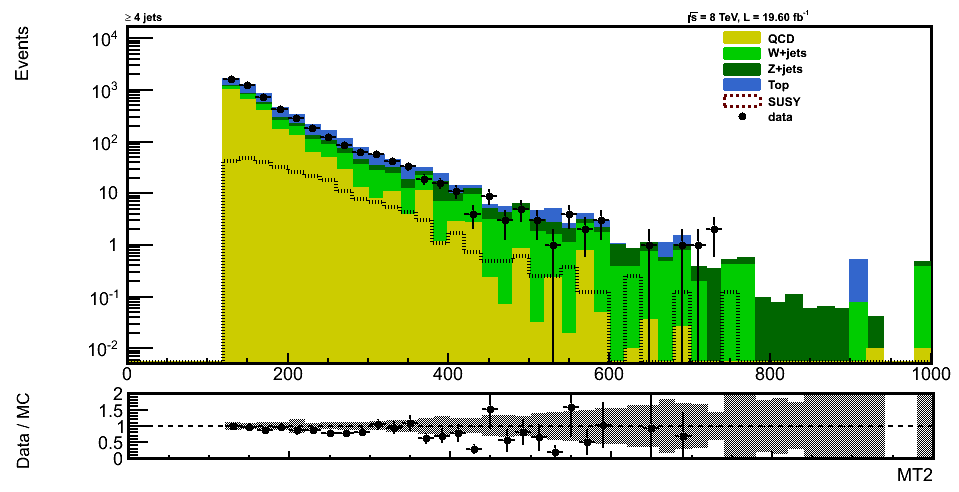
\includegraphics[angle=00,width=0.5\textwidth]{figs/MT2-cut(MT2+trig+VSPT).png}\\
  \mbox{\small{(a)}} & \mbox{\small{(b)}} \\
\end{array}$
\end{center}
\caption{Distribution of \mttwo before(a) and after(b) applying VSPT $< 70$}
\label{fig:MT2VSPT}
\end{figure}

\begin{figure}[!h]
\begin{center}$
\begin{array}{cc} 
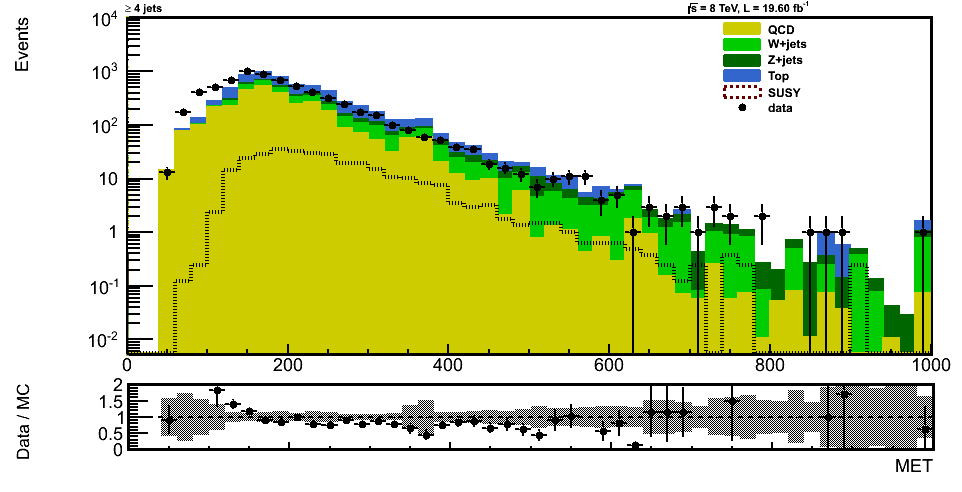
\includegraphics[angle=00,width=0.5\textwidth]{figs/MET-cut(MT2+trig).png}&
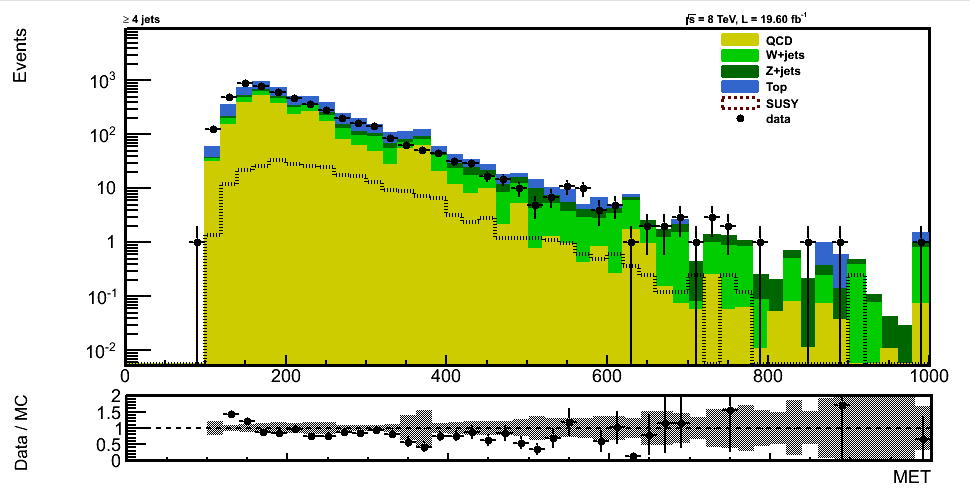
\includegraphics[angle=00,width=0.5\textwidth]{figs/MET-cut(MT2+trig+VSPT).png}\\
	\mbox{\small{(a)}} & \mbox{\small{(b)}} \\
\end{array}$
\end{center}
\caption{Distribution of \met before(a) and after(b) applying VSPT $< 70$}
\label{fig:METVSPT}
\end{figure}

\begin{figure}[!Hhtb]
\begin{center}$
\begin{array}{cc} 
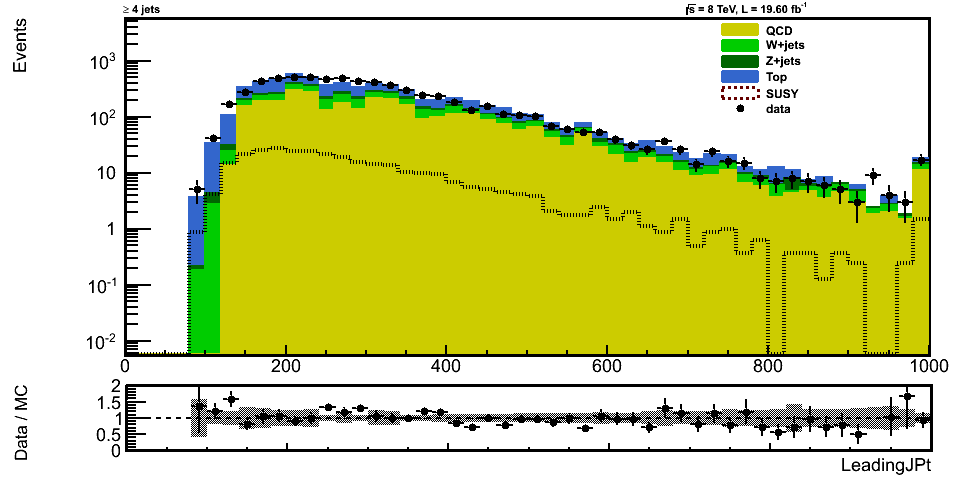
\includegraphics[angle=00,width=0.5\textwidth]{figs/LeadJPt-cut(MT2+trig).png}&
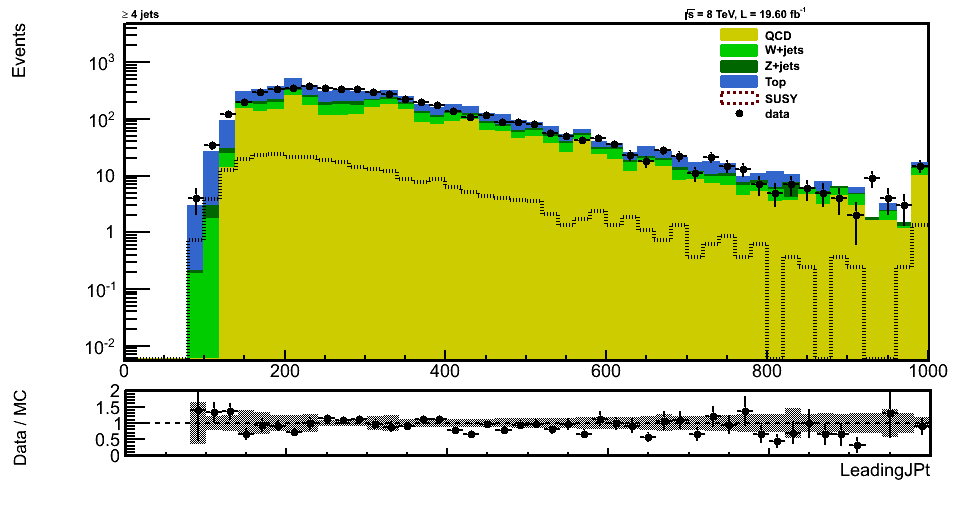
\includegraphics[angle=00,width=0.5\textwidth]{figs/LeadJPt-cut(MT2+trig+VSPT).png}\\
	\mbox{\small{(a)}} & \mbox{\small{(b)}} \\
\end{array}$
\end{center}
\caption{Distribution of Leading Jet $P_{t}$ before(a) and after(b) applying VSPT $< 70$}
\label{fig:LeadJetPtVSPT}
\end{figure}

\begin{figure}[!Hhtb]
\begin{center}$
\begin{array}{cc} 
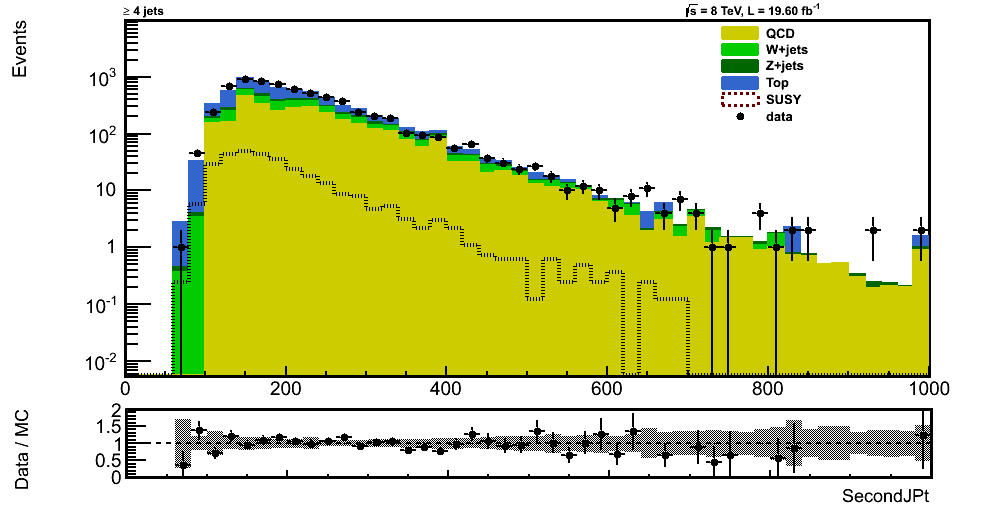
\includegraphics[angle=00,width=0.5\textwidth]{figs/SecJPt-cut(MT2+trig).png}&
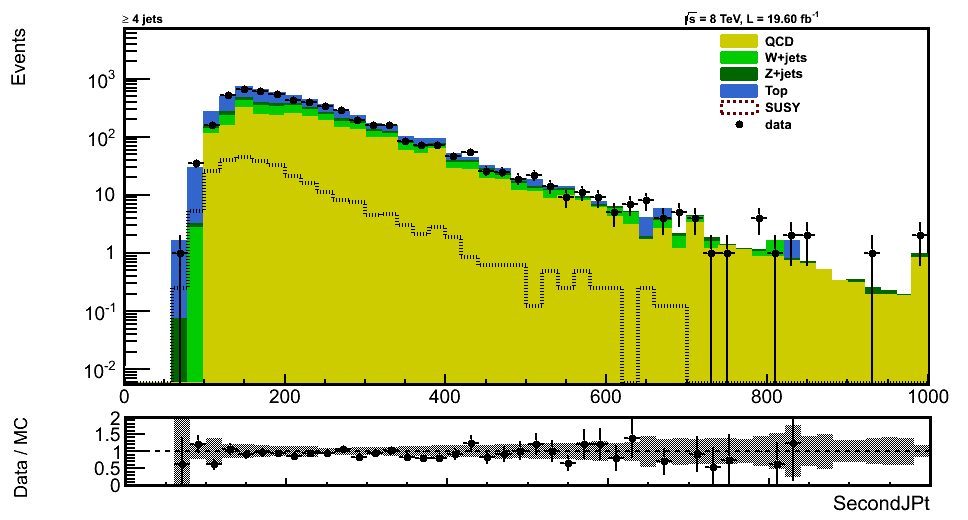
\includegraphics[angle=00,width=0.5\textwidth]{figs/SecJPt-cut(MT2+trig+VSPT).png}\\
	\mbox{\small{(a)}} & \mbox{\small{(b)}} \\
\end{array}$
\end{center}
\caption{Distribution of Second Jet $P_{t}$ before(a) and after(b) applying VSPT $< 70$}
\label{fig:SecJetPtVSPT}
\end{figure}

\begin{figure}[!Hhtb]
\begin{center}$
\begin{array}{cc} 
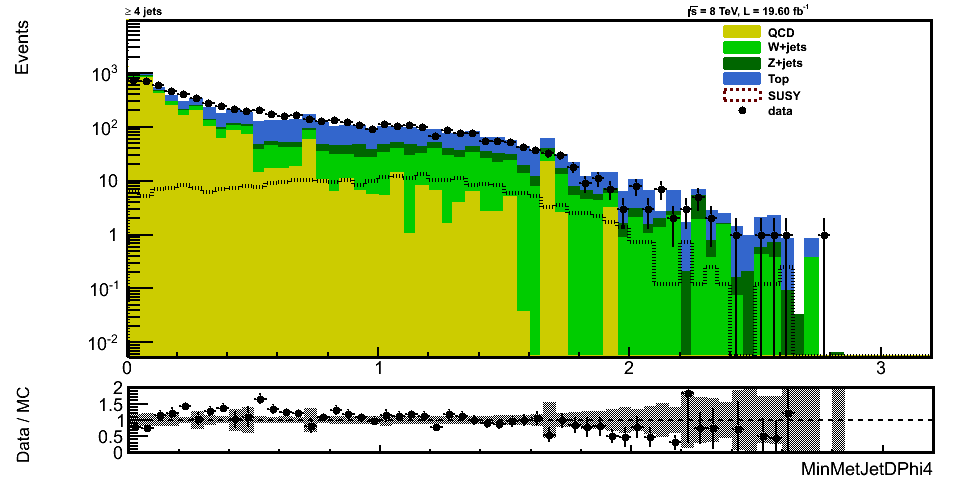
\includegraphics[angle=00,width=0.5\textwidth]{figs/MinDPhi-cut(MT2+trig).png}&
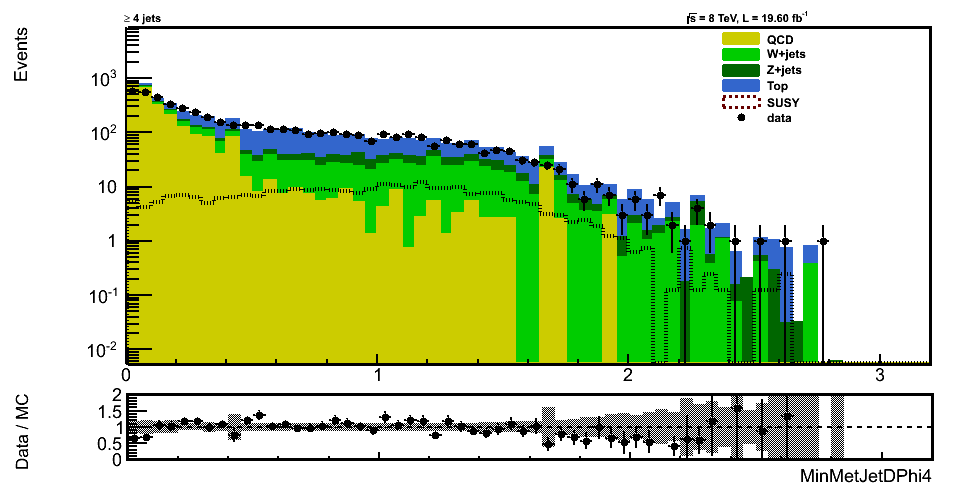
\includegraphics[angle=00,width=0.5\textwidth]{figs/MinDPhi-cut(MT2+trig+VSPT).png}\\
	\mbox{\small{(a)}} & \mbox{\small{(b)}} \\
\end{array}$
\end{center}
\caption{Distribution of \mindphifour before(a) and after(b) applying VSPT $< 70$}
\label{fig:MinDPhiVSPT}
\end{figure}

\begin{figure}[!Hhtb]
\begin{center}$
\begin{array}{cc} 
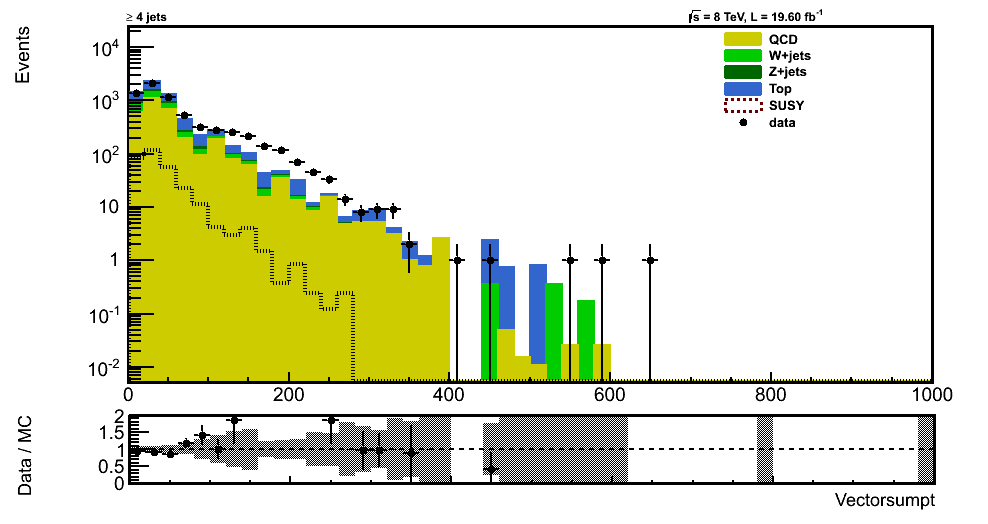
\includegraphics[angle=00,width=0.5\textwidth]{figs/VSPT-cut(MT2+trig).png}&
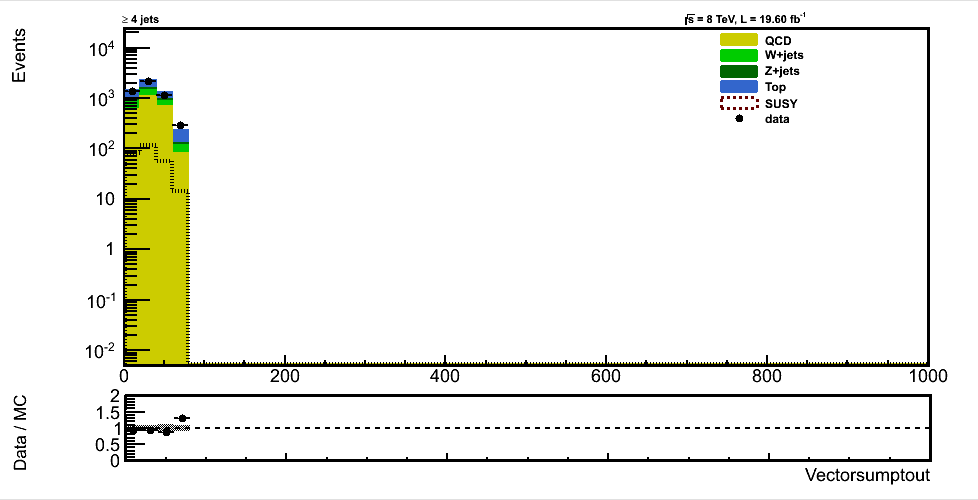
\includegraphics[angle=00,width=0.5\textwidth]{figs/VSPT-cut(MT2+trig+VSPT).png}\\
	\mbox{\small{(a)}} & \mbox{\small{(b)}} \\
\end{array}$
\end{center}
\caption{Distribution of VSPT before(a) and after(b) applying VSPT $< 70$}
\label{fig:VSPTVSPT}
\end{figure}


To justify the cut on \mindphifour which is $\mindphifour > 0.3$, like VSPT, We looked at the distributions of different variables before and after applying $\mindphifour > 0.3$ when the other cuts 
except $\mttwo > 125 $ were relaxed. As it is obvious from figures \ref{fig:MT2MinDPhi}-\ref{fig:VSPTMinDPhi}, 
by applying $\mindphifour > 0.3$ we have a better agreement 
between data and MC, 

\begin{figure}[!Hhtb]
\begin{center}$
\begin{array}{cc} 
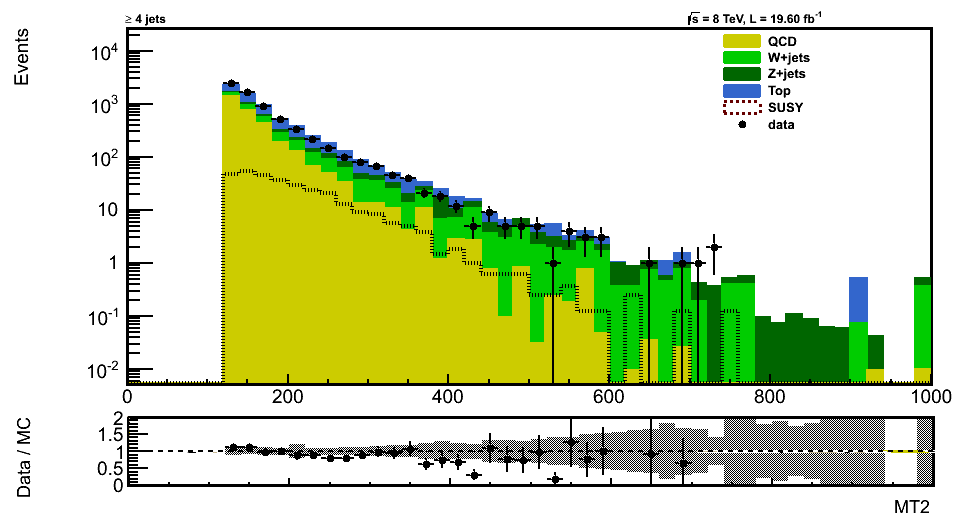
\includegraphics[angle=00,width=0.5\textwidth]{figs/MT2-cut(MT2+trig).png}&
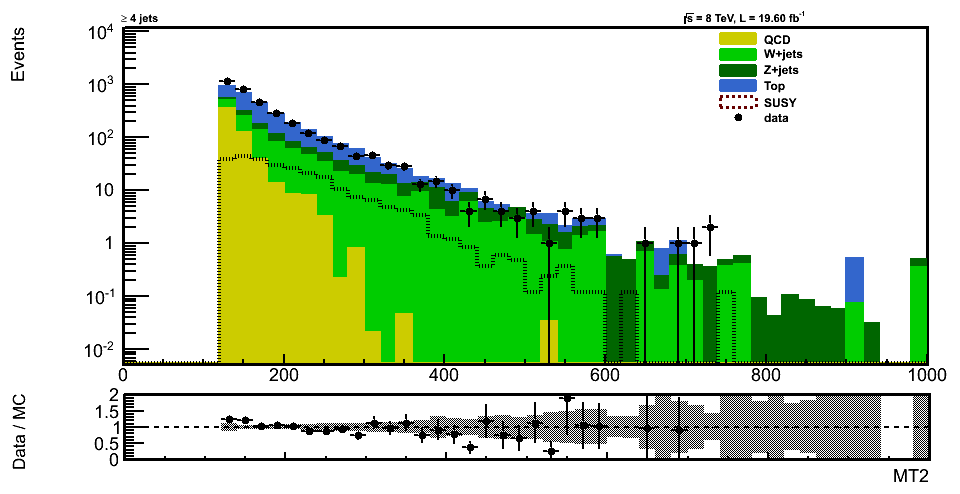
\includegraphics[angle=00,width=0.5\textwidth]{figs/MT2-cut(MT2+trig+MinDPhi).png}\\
	\mbox{\small{(a)}} & \mbox{\small{(b)}} \\
\end{array}$
\end{center}
\caption{Distribution of \mttwo before(a) and after(b) applying $\mindphifour > 0.3$}
\label{fig:MT2MinDPhi}
\end{figure}

\begin{figure}[!Hhtb]
\begin{center}$
\begin{array}{cc} 
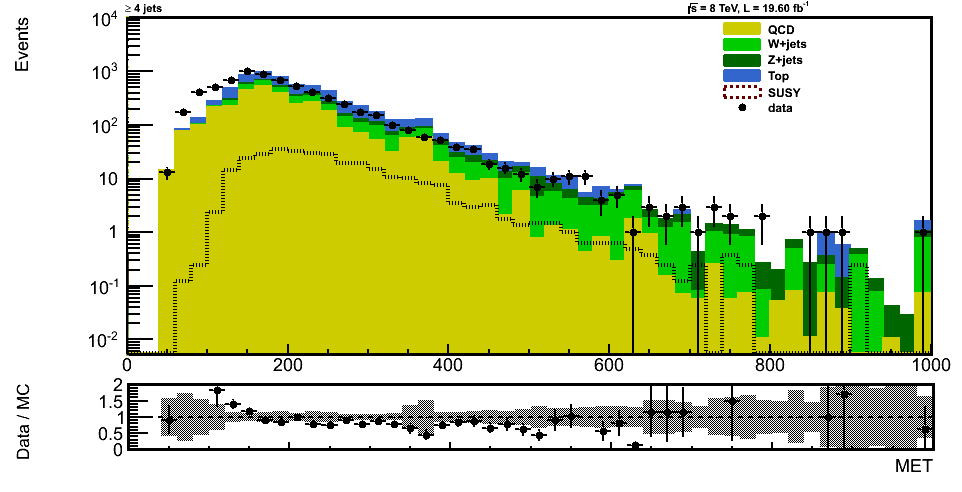
\includegraphics[angle=00,width=0.5\textwidth]{figs/MET-cut(MT2+trig).png}&
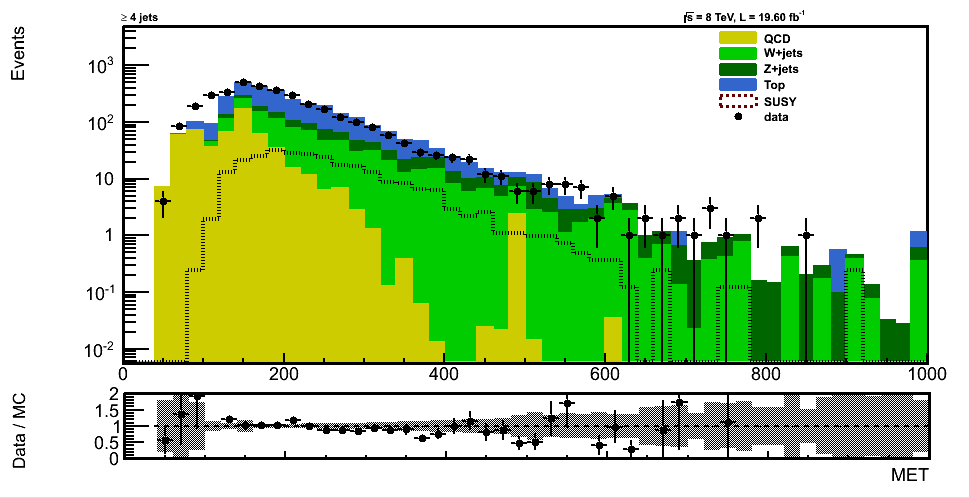
\includegraphics[angle=00,width=0.5\textwidth]{figs/MET-cut(MT2+trig+MinDPhi).png}\\
	\mbox{\small{(a)}} & \mbox{\small{(b)}} \\
\end{array}$
\end{center}
\caption{Distribution of \met before(a) and after(b) applying $\mindphifour > 0.3$}
\label{fig:METMinDPhi}
\end{figure}

\begin{figure}[!Hhtb]
\begin{center}$
\begin{array}{cc} 
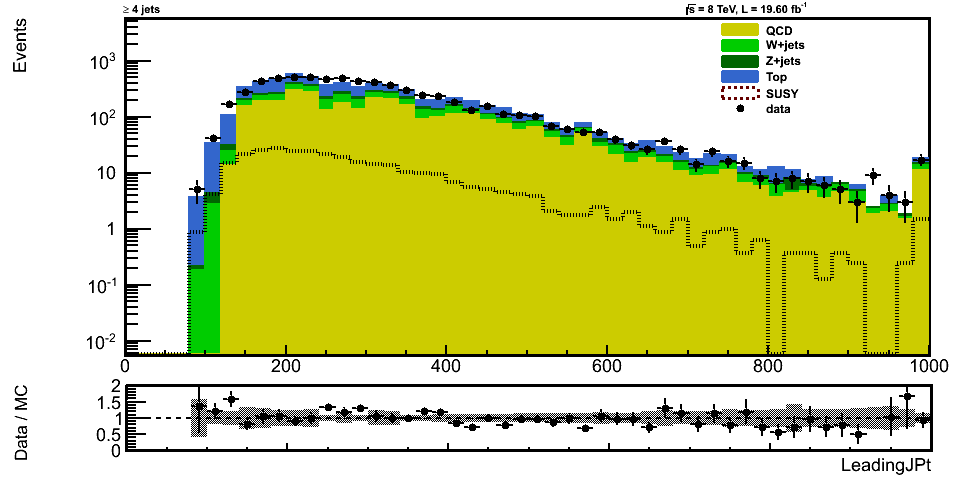
\includegraphics[angle=00,width=0.5\textwidth]{figs/LeadJPt-cut(MT2+trig).png}&
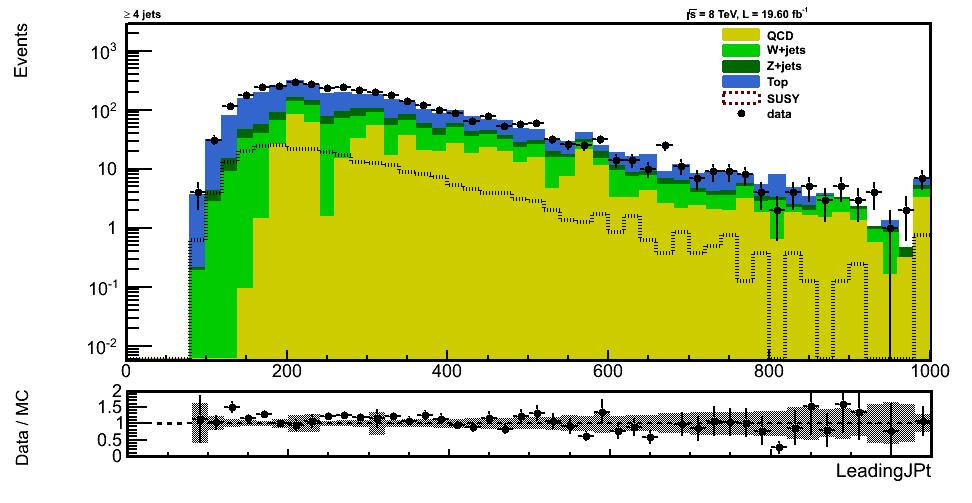
\includegraphics[angle=00,width=0.5\textwidth]{figs/LeadJPt-cut(MT2+trig+MinDPhi).png}\\
	\mbox{\small{(a)}} & \mbox{\small{(b)}} \\
\end{array}$
\end{center}
\caption{Distribution of Leading Jet $P_{T}$ before(a) and after(b) applying $\mindphifour > 0.3$}
\label{fig:LeadJetPtMinDPhi}
\end{figure}

\begin{figure}[!Hhtb]
\begin{center}$
\begin{array}{cc} 
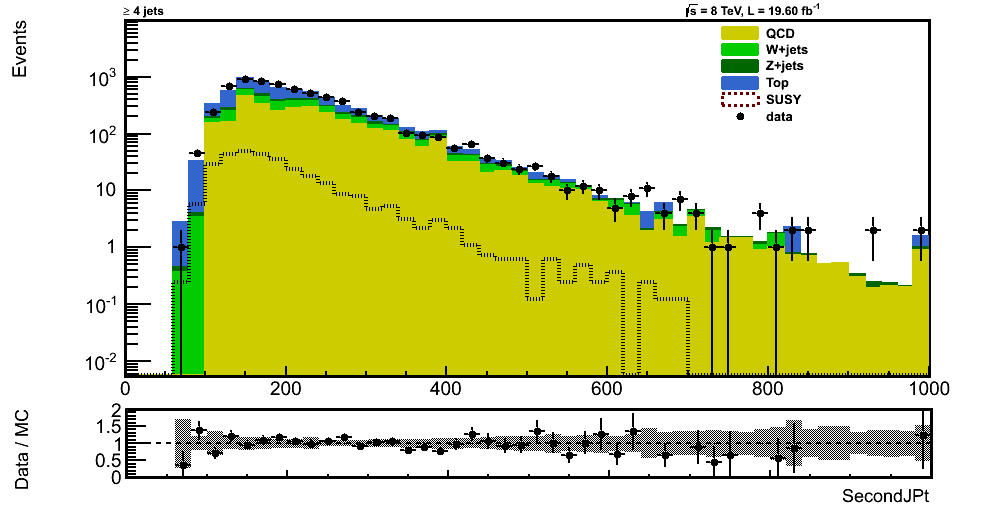
\includegraphics[angle=00,width=0.5\textwidth]{figs/SecJPt-cut(MT2+trig).png}&
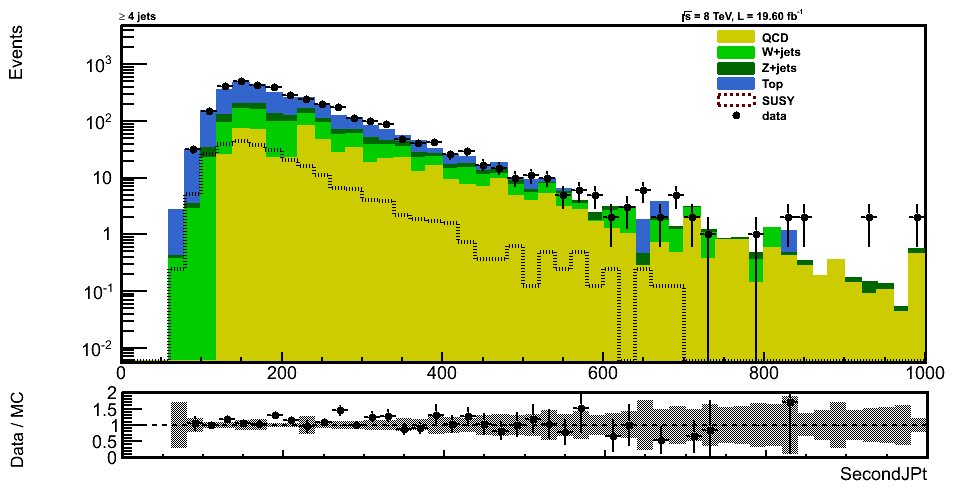
\includegraphics[angle=00,width=0.5\textwidth]{figs/SecJPt-cut(MT2+trig+MinDPhi).png}\\
%	\mbox{\small{(a)}} & \mbox{\small{(b)}} \\
\end{array}$
\end{center}
\caption{Distribution of Second Jet $P_{T}$ before(a) and after(b) applying $\mindphifour > 0.3$}
\label{fig:SecJetPtMinDPhi}
\end{figure}

\begin{figure}[!Hhtb]
\begin{center}$
\begin{array}{cc} 
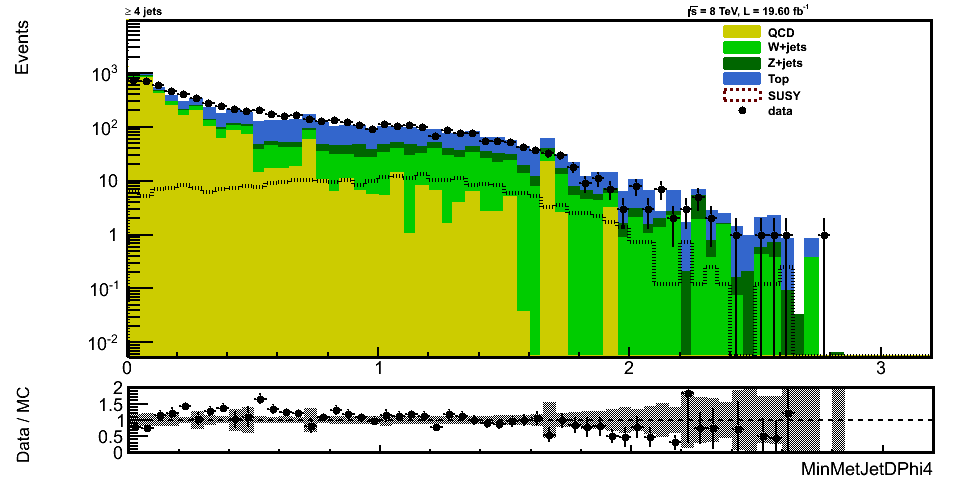
\includegraphics[angle=00,width=0.5\textwidth]{figs/MinDPhi-cut(MT2+trig).png}&
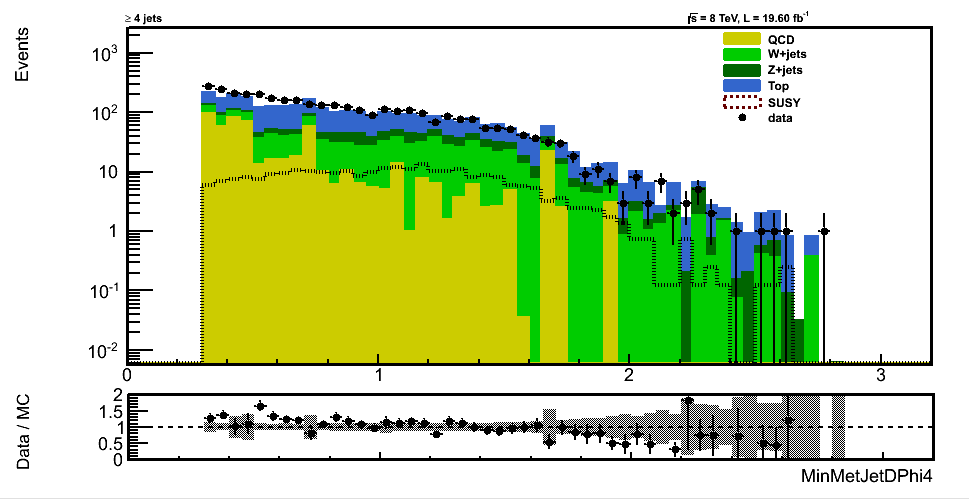
\includegraphics[angle=00,width=0.5\textwidth]{figs/MinDPhi-cut(MT2+trig+MinDPhi).png}\\
	\mbox{\small{(a)}} & \mbox{\small{(b)}} \\
\end{array}$
\end{center}
\caption{Distribution of \mindphifour before(a) and after(b) applying $\mindphifour > 0.3$}
\label{fig:MinDPhiMinDPhi}
\end{figure}

\begin{figure}[!Hhtb]
\begin{center}$
\begin{array}{cc} 
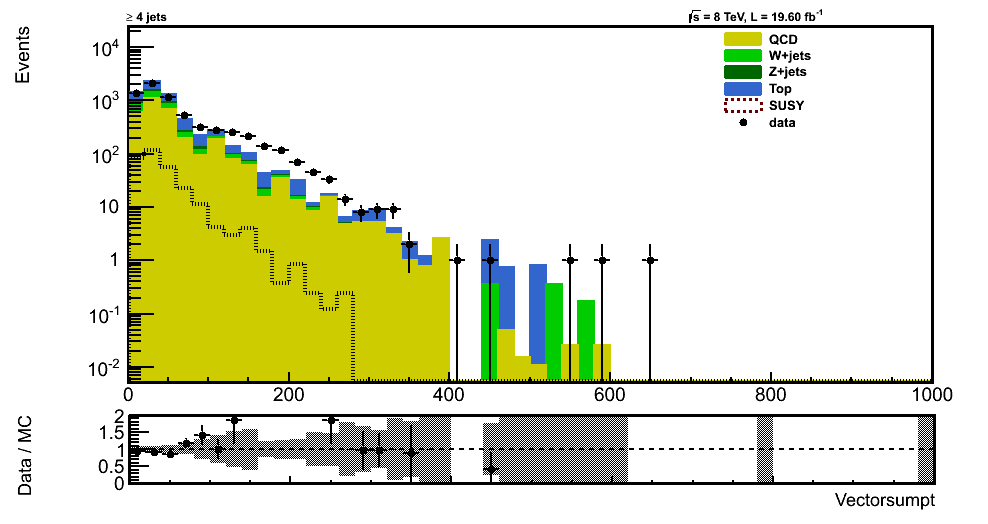
\includegraphics[angle=00,width=0.5\textwidth]{figs/VSPT-cut(MT2+trig).png}&
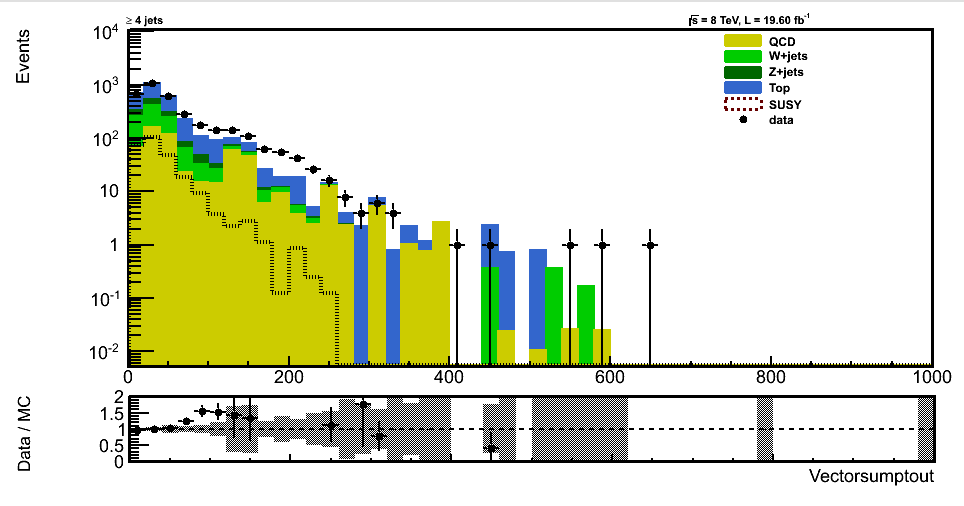
\includegraphics[angle=00,width=0.5\textwidth]{figs/VSPT-cut(MT2+trig+MinDPhi).png}\\
	\mbox{\small{(a)}} & \mbox{\small{(b)}} \\
\end{array}$
\end{center}
\caption{Distribution of VSPT before(a) and after(b) applying $\mindphifour > 0.3$}
\label{fig:VSPTMinDPhi}
\end{figure}


We applied Jet-Met smearing on MC samples and then plotted the distributions of \met and \mttwo. As it is seen below
there is an excellent agreement between Data and MC in both cases.

\begin{figure}[!Hhtb]
\begin{center}$
\begin{array}{cc} 
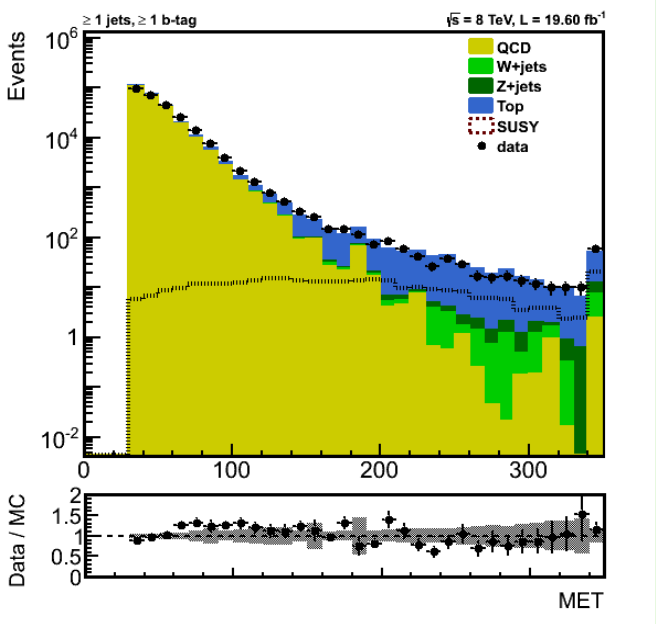
\includegraphics[angle=00,width=0.5\textwidth]{figs/MET-before-JMS.png}&
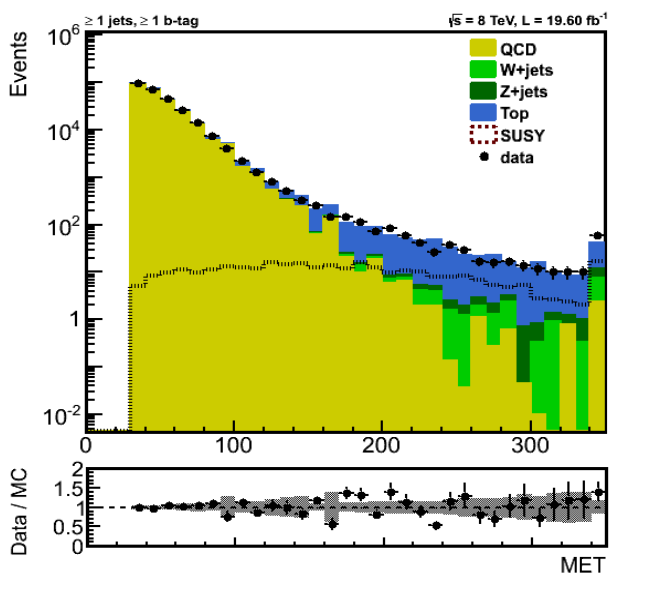
\includegraphics[angle=00,width=0.5\textwidth]{figs/MET-after-JMS.png}\\
	\mbox{\small{(a)}} & \mbox{\small{(b)}} \\
\end{array}$
\end{center}
\caption{Distribution of \met before(a) and after(b) applying Jet-MET smearing}
\label{fig:METJetMETSmear}
\end{figure}


\begin{figure}[!Hhtb]
\begin{center}$
\begin{array}{cc} 
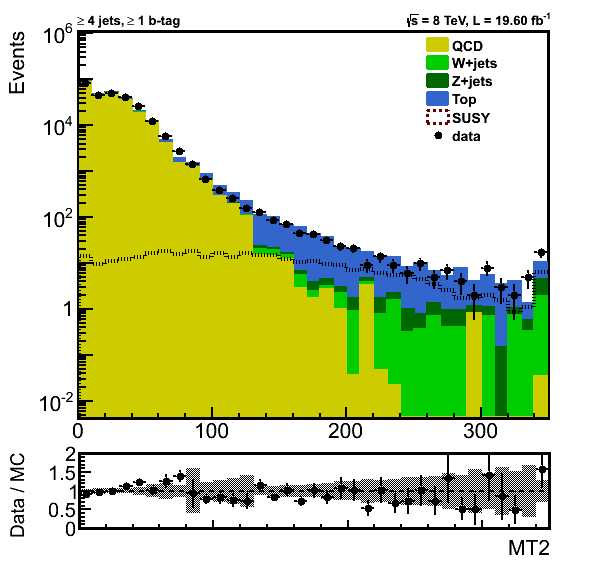
\includegraphics[angle=00,width=0.5\textwidth]{figs/MT2-before-JMS.png}&
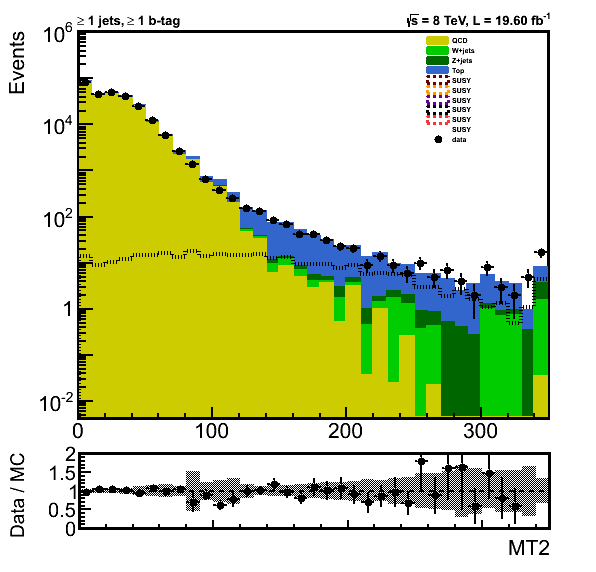
\includegraphics[angle=00,width=0.5\textwidth]{figs/MT2-after-JMS.png}\\
	\mbox{\small{(a)}} & \mbox{\small{(b)}} \\
\end{array}$
\end{center}
\caption{Distribution of \mttwo before(a) and after(b) applying Jet-MET smearing}
\label{fig:MT2JetMETSmear}
\end{figure}

We also applied pile-up reweighting and b-tagging scale factor alongside of Jet-MET smearing and to see that these 
effects are under control and doing their jobs, we looked at the number of CSVT b jets, and it is clear that there is an 
excellent consistency between data and MC,


\begin{figure}[!Hhtb]
\begin{center}$
\begin{array}{cc} 
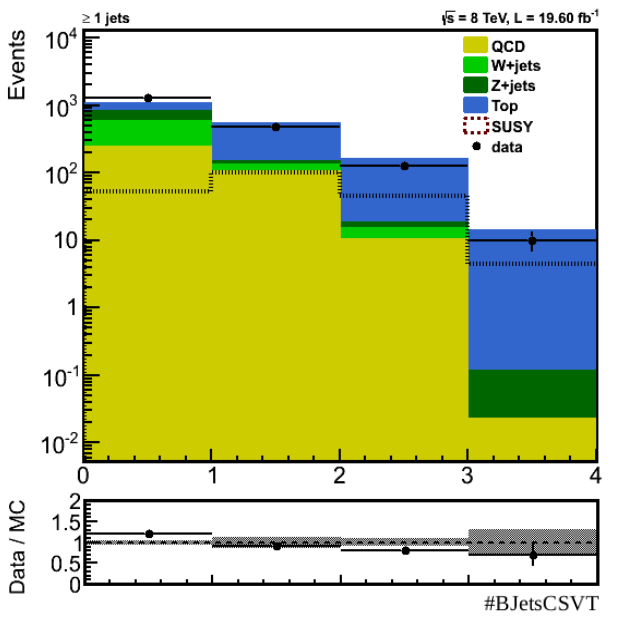
\includegraphics[angle=00,width=0.5\textwidth]{figs/NB-noSF-noPU-noJMS.png}&
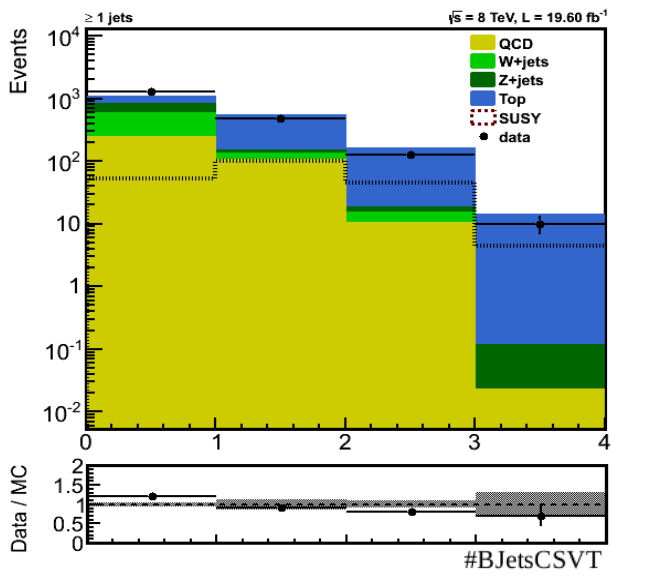
\includegraphics[angle=00,width=0.5\textwidth]{figs/NB-noSF-noPU-JMS.png}\\
	\mbox{\small{(a).no scale factor,no pile-up, no Jet-MET smearing}} & \mbox{\small{(b).no scale factor,no pile-up,Jet-MET smeared}} \\
\end{array}$
\end{center}
\begin{center}$
\begin{array}{cc}
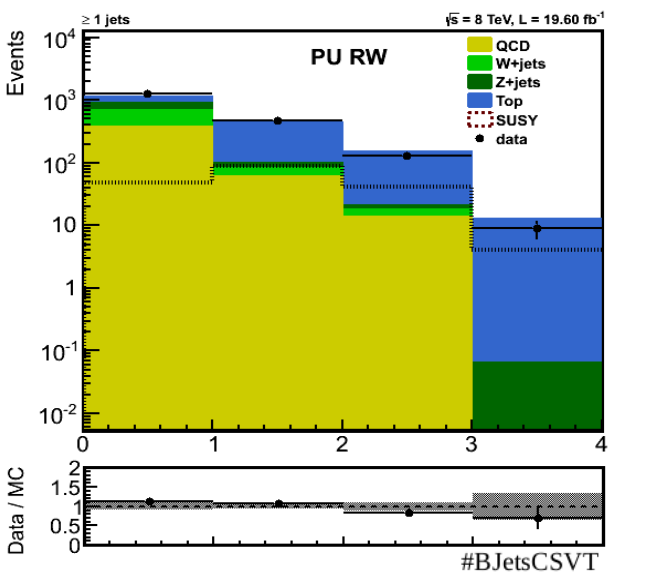
\includegraphics[angle=00,width=0.5\textwidth]{figs/NB-noSF-PU-JMS.png}&
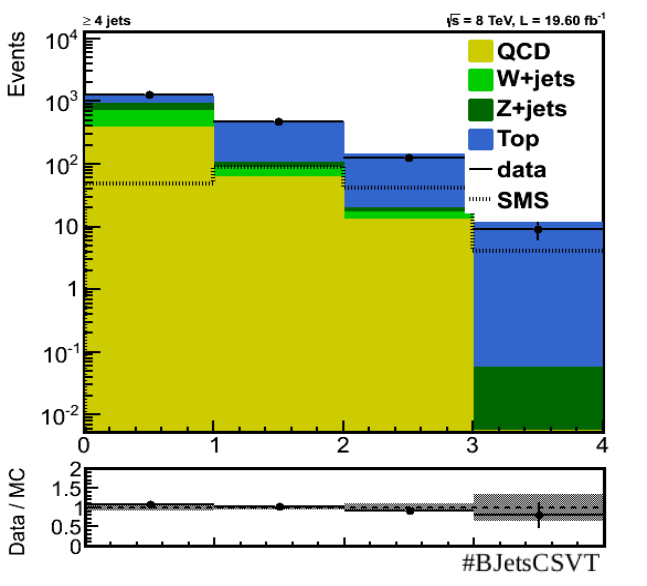
\includegraphics[angle=00,width=0.5\textwidth]{figs/NB-SF-PU-JMS.png}\\
	\mbox{\small{(c).no scale factor,pile-up reweighted,Jet-MET smeared}} & \mbox{\small{(d.scale factor applied
	,pile-up reweighted,Jet-MET smeared)}} \\
\end{array}$
\end{center}
\caption{Effects of applying Jet-MET smearing, pile-up reweighting and b-tagging scale factor on distribution of number of CSVT b jets}
\label{fig:NBCSVTPileUpJetMETSmearSF}
\end{figure}

It was also checked the correlation of between variables \mttwo and \met for different samples. It is seen that 
there is a correlation betwwn these two variables and events having hight \met sit in the high \mttwo region.  
\begin{figure}[!Hhtb]
\begin{center}$
\begin{array}{ccc} 
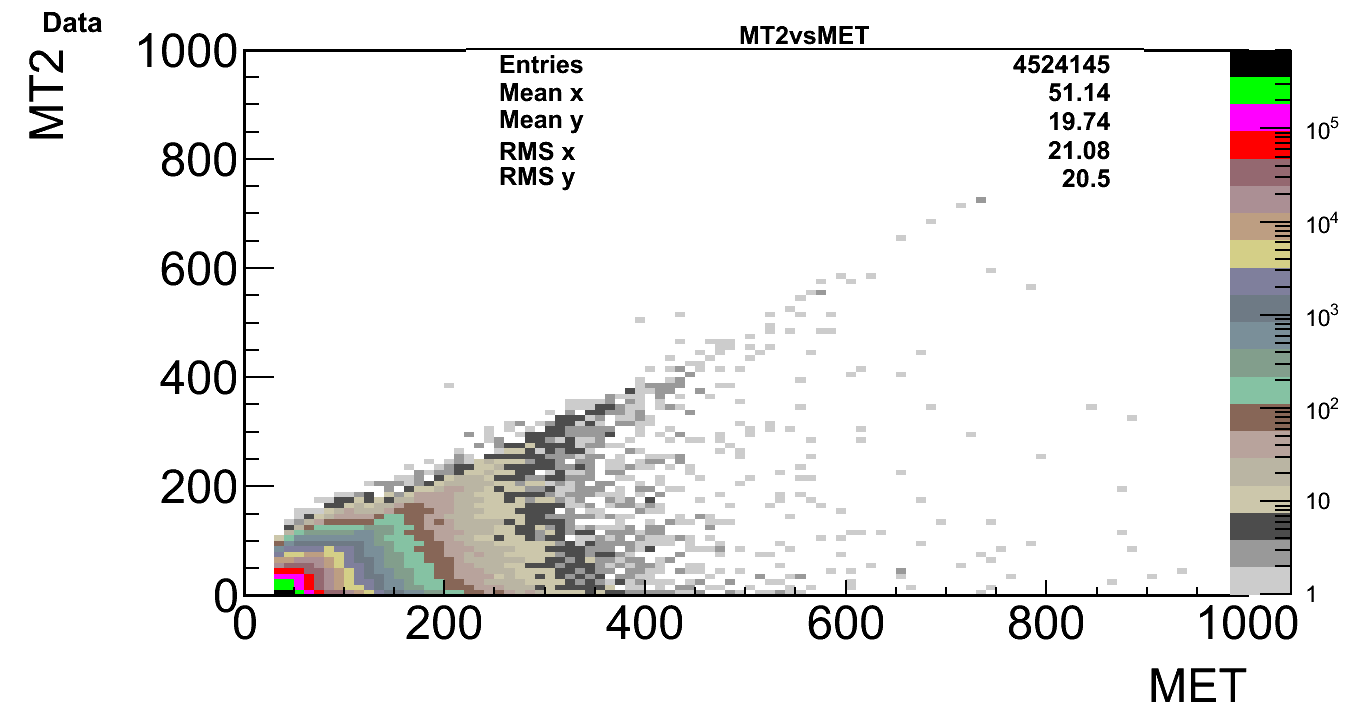
\includegraphics[angle=00,width=0.5\textwidth]{figs/MT2-MET-before-AllCuts--Data.png}&
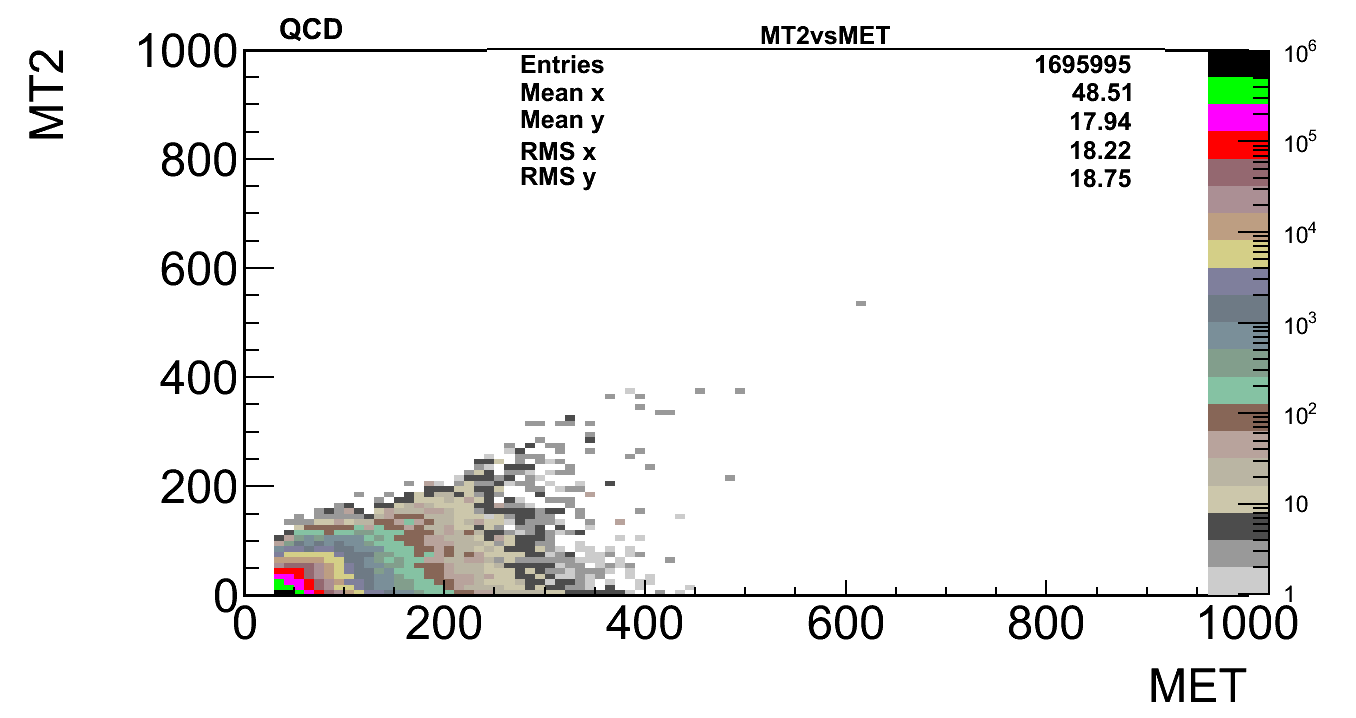
\includegraphics[angle=00,width=0.5\textwidth]{figs/MT2-MET-before-AllCuts-QCD.png}&
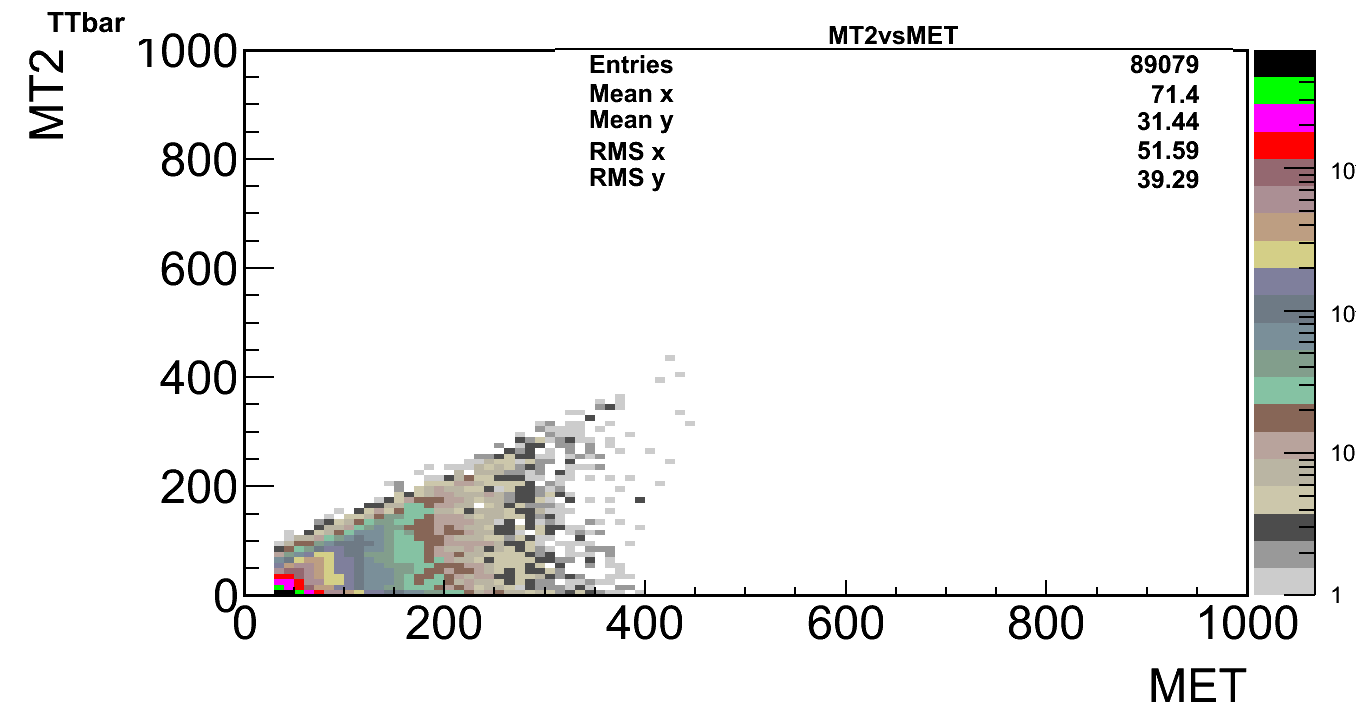
\includegraphics[angle=00,width=0.5\textwidth]{figs/MT2-MET-before-AllCuts-Top.png}\\
	\mbox{\small{(a).data sample}} & \mbox{\small{(b).QCD sample}} & \mbox{\small{(c).top sample}}\\
\end{array}$
\end{center}
\caption{Scatter plot of \met and \mttwo}
\label{fig:MT2METCorr}
\end{figure}

To figure out the effects of pile-up reweighting, it was plotted the number of vertices before and after pile-up reweighting for data and MC samples which as it is seen below, this reweighting has no effecs on data but MC has been affected.

\begin{figure}[!Hhtb]
\begin{center}$
\begin{array}{cc} 
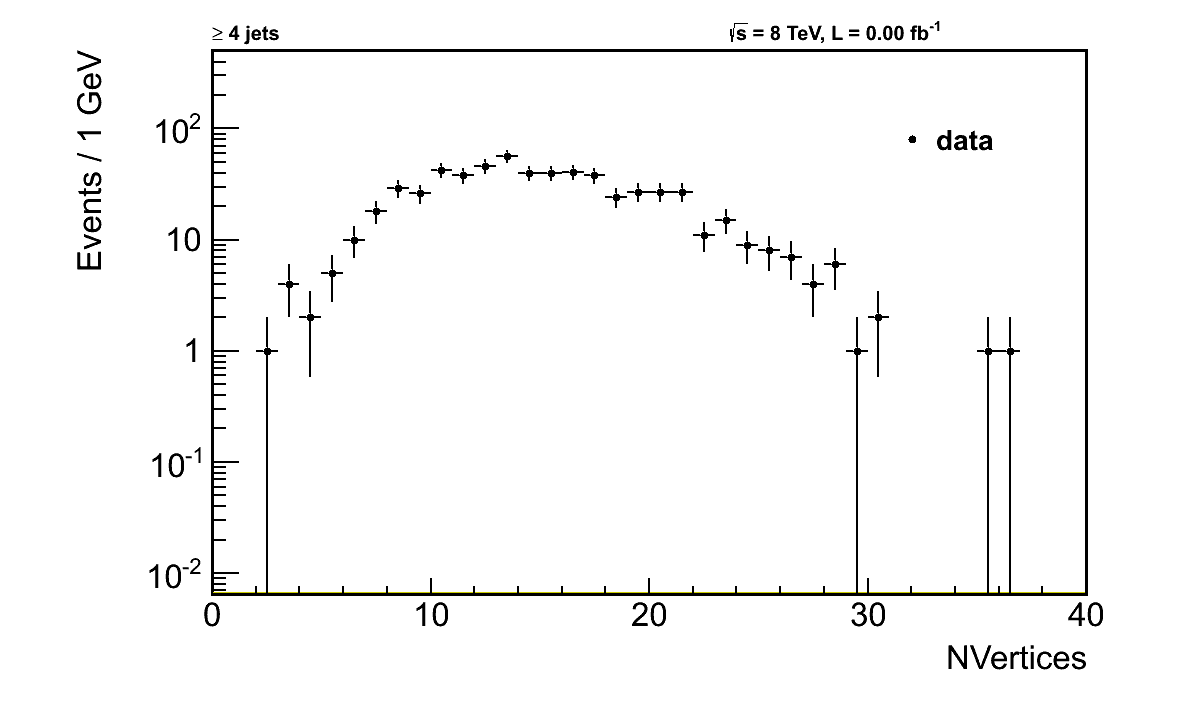
\includegraphics[angle=00,width=0.5\textwidth]{figs/NVertices-Data-NoPU-NoRatio.png}&
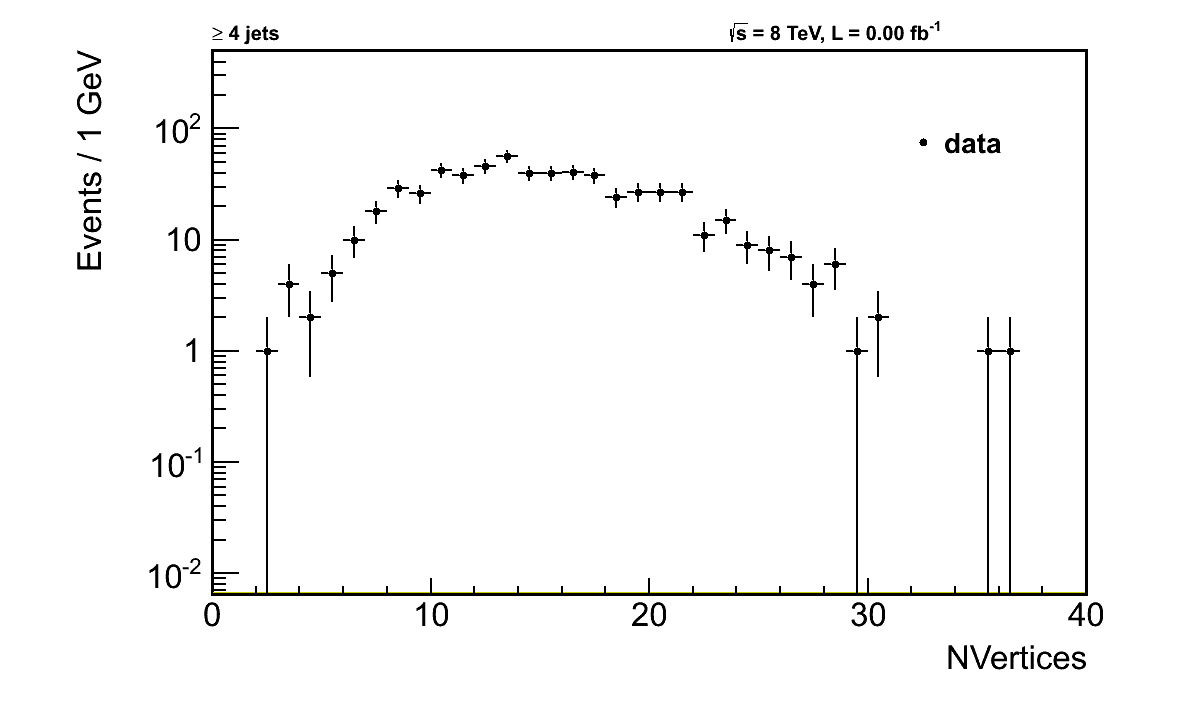
\includegraphics[angle=00,width=0.5\textwidth]{figs/NVertices-Data-PU-NoRatio.png}\\
	\mbox{\small{(a)}} & \mbox{\small{(b)}} \\
\end{array}$
\end{center}
\caption{Distribution of number of vertices for data before(a) and after(b) pile-up reweighting}
\label{fig:NVerticesPileUpData}
\end{figure}
\begin{figure}[!Hhtb]
\begin{center}$
\begin{array}{ccc} 
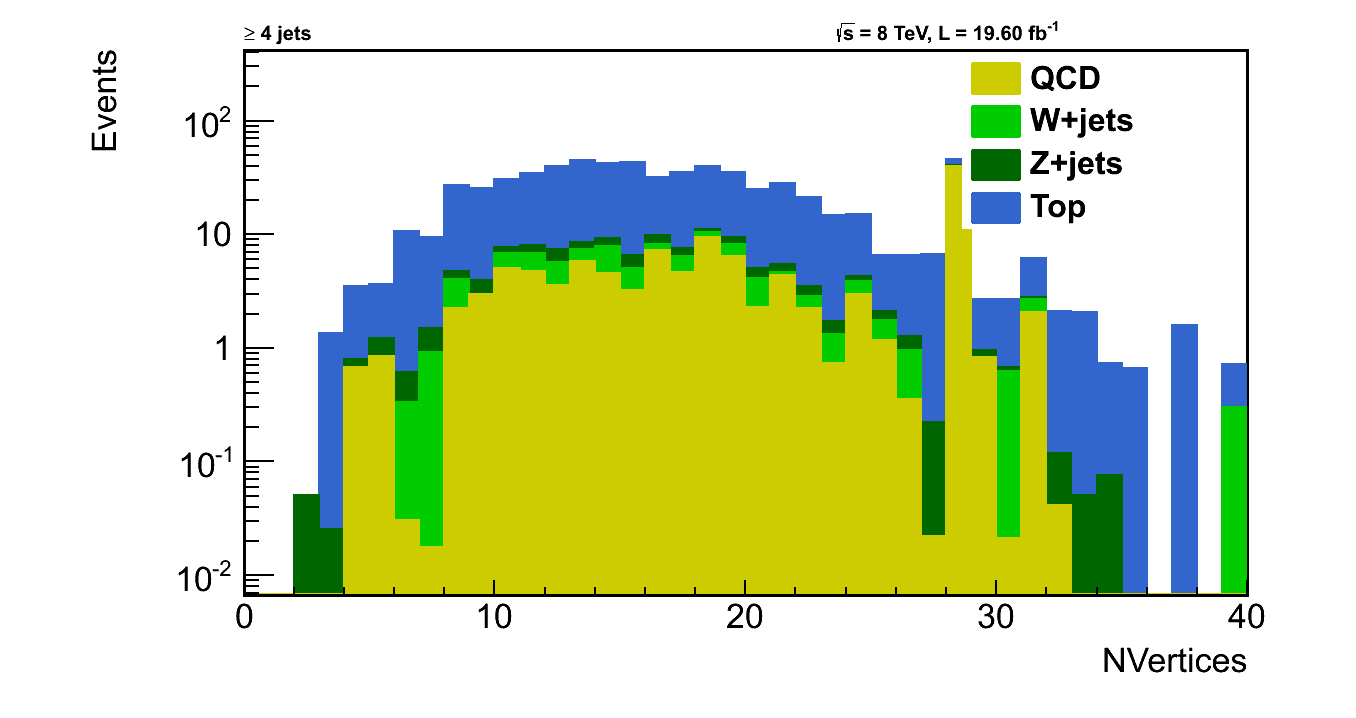
\includegraphics[angle=00,width=0.5\textwidth]{figs/NVertices-MC-NoPU-NoRatio.png}&
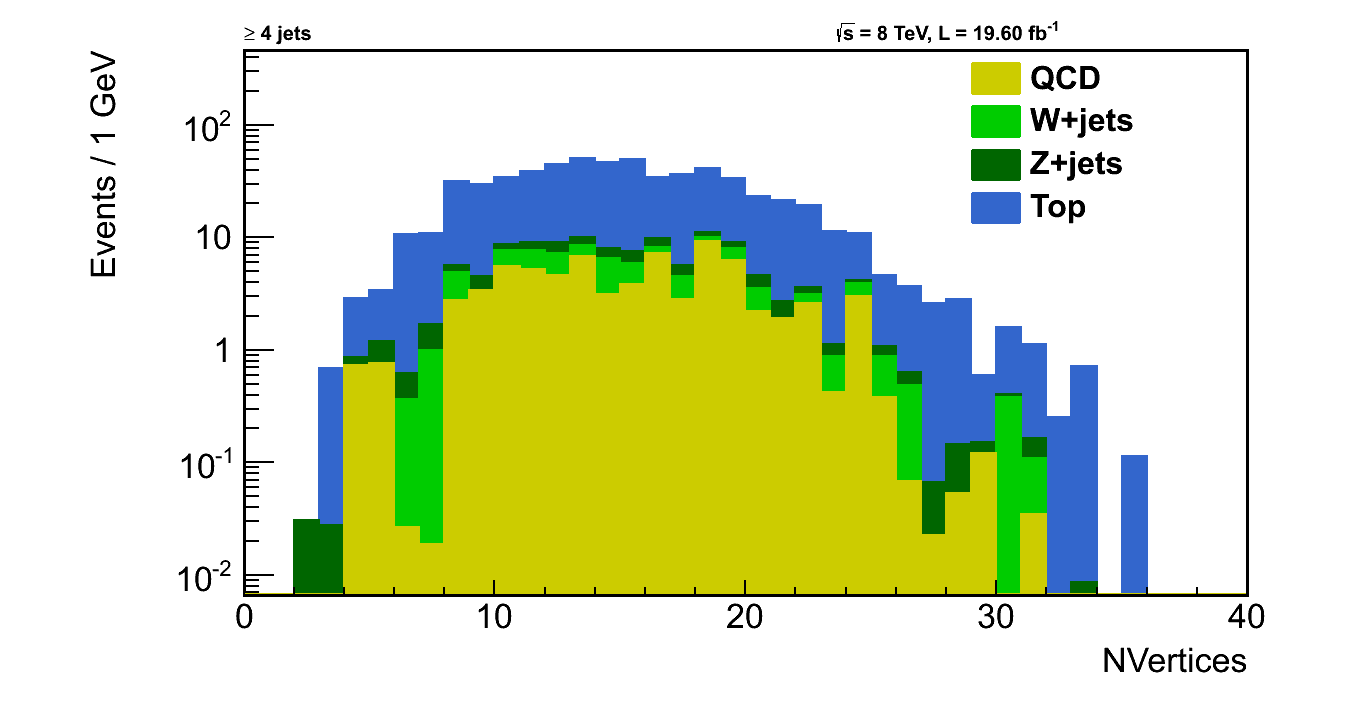
\includegraphics[angle=00,width=0.5\textwidth]{figs/NVertices-MC-PU-NoRatio.png}\\
	\mbox{\small{(a)}} & \mbox{\small{(b)}} \\
\end{array}$
\end{center}
\caption{Distribution of number of vertices for MC before(a) and after(b) pile-up reweighting }
\label{fig:NVerticesPileUpMC}

\end{figure}
